\section{Construtor e destrutor}


\begin{frame}{Passagem de parâmetros para um construtor}
\begin{figure}
\centering
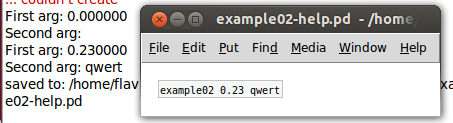
\includegraphics[width=0.7\textwidth]{example2}
\end{figure}
\end{frame}


\begin{frame}[fragile]{Exemplo de construtor com passagem de parâmetros}
\begin{lstlisting}
// Constructor of the class
void *example2_new(t_symbol * arg1, t_floatarg arg2) {
    t_example2 *x = (t_example2 *) pd_new(example2_class);
    post("First arg: %s", arg1->s_name);
    post("Second arg: %f", arg2);
    return (void *) x;
}

void example2_setup(void) {
    example2_class = class_new(gensym("example2"),
            (t_newmethod) example2_new, // Constructor
            0,
            sizeof (t_example2),
	    CLASS_NOINLET,
            A_DEFFLOAT, // Constructor parameter 1
            A_DEFSYMBOL, // Constructor parameter 2
            0);
}
\end{lstlisting}
\end{frame}


\begin{frame}{Outros tipos de átomo}
Existem diversos tipos de átomo definidos pelo arquivo \texttt{m\_pd.h} que
podem ser utilizados na passagem de parâmetros:
\begin{itemize}
\item A\_NULL,
\item A\_FLOAT,
\item A\_SYMBOL,
\item A\_POINTER,
\item A\_SEMI,
\item A\_COMMA,
\item A\_DEFFLOAT,
\item A\_DEFSYM,
\item A\_DOLLAR, 
\item A\_DOLLSYM,
\item A\_GIMME,
\item A\_CANT
\end{itemize}
\end{frame}


\begin{frame}[fragile]{Exemplo de construtor utilizando \texttt{A\_GIMME}}
\begin{lstlisting}
// Constructor of the class
void *example9_new(t_symbol *s,
                    int argc, t_atom * argv) {
   t_example9 *x = (t_example9 *) pd_new(example9_class);
   post("%d parameters received",argc);
   return (void *) x;
}

void example9_setup(void) {
   example9_class = class_new(gensym("example9"),
     (t_newmethod) example9_new, // Constructor
     (t_method) example9_destroy, // Destructor
     sizeof (t_example9),
     CLASS_NOINLET,
     A_GIMME, // Allows various parameters
     0); // LAST argument is ALWAYS zero
}
\end{lstlisting}
\end{frame}


\begin{frame}{Exemplo de construtor com diferentes parâmetros}
\begin{figure}[h!]
\centering
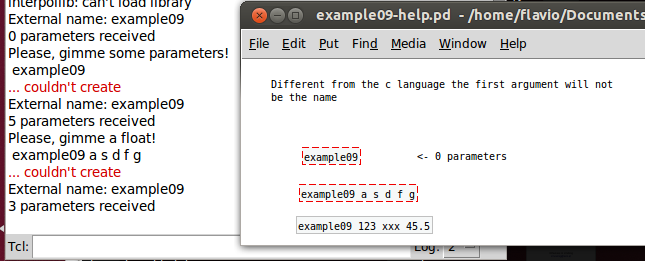
\includegraphics[width=0.7\textwidth]{example9}
\caption{Diferente da linguagem C, o primeiro parâmetro não é o nome do external.}
\end{figure}
\end{frame}


\begin{frame}[fragile]{Exemplo de destrutor}
\begin{lstlisting}
// Destroy the object
void example9_destroy(t_example9 *x) {
  post("You say good bye and I say hello");
}

void example9_setup(void) {
   example9_class = class_new(gensym("example9"),
     (t_newmethod) example9_new, // Constructor
     (t_method) example9_destroy, // Destructor
     sizeof (t_example9),
     CLASS_NOINLET,
     A_GIMME, // Allows various parameters
     0); // LAST argument is ALWAYS zero
}
\end{lstlisting}
Para liberar memória, podemos utilizar:
\begin{lstlisting}
void freebytes(void *x, size_t nbytes)
\end{lstlisting}
\end{frame}

